\subsection{Principe de l'achievement1}
Le but de cet achievement est de ne plus lancer des missiles aléatoires mais de calculer la distance de la cible la plus proche d'un bateau. C'est à dire on doit chercher la case adverse la plus proche en partant d'une case de notre bateau sans dépasser une certaine distance. Dans cet achievement on va considérer que notre torpille peut passer sur des cases où sont présent des bateaux alliés ou adverses.\\
Pour réaliser ceci il va nous falloir calculer toutes les distances de notre position aux positions adverses.
\subsection{Fonctionnement de l'achievement1}
Pour cet achievement on a du rajouter à notre structure Joueur un tableau de position contenant toutes les cases des bateaux qui sont toujours en vie ainsi qu'un entier qui est le nombre de case qui sont toujours en vie. De plus on a du modifier notre fonction oblitérer une case pour mettre la position qui vient d'être oblitérée à la fin du tableau qui liste les cases en vie ainsi que réduire la taille de 1.\\
De plus, on a créer deux constantes qui sont :
\begin{itemize}
\item {\textit{NB\_COUP\_MAX}} qui nous dit le nombre maximum de tour de boucle que notre programme va réaliser.
\item {\textit{PORTEE\_MAX\_TORPILLE}} qui est la distance maximale qu'une torpille peut faire.
\end{itemize}
Pour réaliser cet achievement on va avoir besoin d'une fonction qui exprime la distance entre deux cases et ainsi qu'une fonction qui nous renvoi la position la plus proche de notre position de départ.
\subsubsection{Distance minimale}
Notre fonction de distance minimale a pour prototype :
\begin{lstlisting}
int distance_minimale(struct Position *position1, struct Position *position2);
\end{lstlisting}
Cette fonction applique juste la formule $|p1.ligne - p2.ligne| + |p1.colonne - p2.colonne|$. Ce qui nous permet d'avoir la distance minimale entre deux positions. Cette fonction a pour complexité $\Theta(1)$.
\subsubsection{Arrivée de la torpille}
Cette fonction va rechercher la position la plus proche dans les cases en vie de l'adversaire sans dépasser la distance {\textit{PORTEE\_MAX\_TORPILLE}}. Cette fonction a pour prototype :
\begin{lstlisting}
int arrive_torpille(struct Position *pos_de_depart, struct Joueur *joueur, struct Position *pos_arrive);
\end{lstlisting}
Cette fonction change la position pos\_arrive par la nouvelle position ({\textit{NB\_LIGNES}} et {\textit{NB\_COLONNES}} si ce n'est pas possible). Et nous renvoi un entier qui est la distance parcourue. Cette fonction a pour complexité $\Theta(n)$ où n est le nombre de case en vie du joueur adverse.\\
\subsubsection{Affichage des torpilles}
Cette fonction affiche sur une grille à part le chemin des torpilles avec des flèches pour afficher la direction de la torpille. La "x" est le point de départ et la tête de mort est le point d'arrivé. Ce qui donne sur l'exemple suivant avec un départ en position (2, 0) et une arrivée en (9, 8):\\
\begin{center}
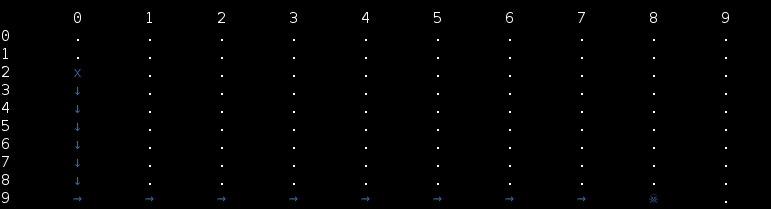
\includegraphics[scale=0.75]{./image/chemin_torpille.png}\\
\end{center}
En SDL on va avoir le chemin des torpilles de la même couleur que le joueur en un peu plus foncé.\\
Pour avoir le chemin, on va partir de la position de départ afin d'aller jusqu'à la position d'arrivée. Premièrement on va diminuer ou augmenter l'indice de ligne de la position de départ pour arriver au même que la position d'arrivée puis on va faire la même chose avec les colonnes.\\
La complexité pour afficher le chemin des torpilles est en $\Theta(n)$ où n est la distance parcourue par la torpille.
\subsubsection{Fonctionnement de la boucle de jeu}
Notre fonction qui fait tourner la boucle de jeu a pour prototype :
\begin{lstlisting}
int achievement1(SDL_Surface *ecran, int affichage);
\end{lstlisting}
Elle prend un paramètre un écran si on utilise l'affichage SDL et un entier qui permet de savoir l'affichage souhaité et retourne un entier afin de nous dire le joueur qui a gagné.\\
Notre boucle de jeu tourne tant qu'il reste des bateaux des 2 joueurs et que le nombre de coup n'a pas dépassé la constante {\textit{NB\_COUP\_MAX}}. Dans notre boucle, on va :
\begin{itemize}
\item Calculer la position d'arrivée des torpilles pour les deux joueurs.
\item Oblitérer les cases si la position d'arrivée est possible (ie ne dépasse pas la distance maximale)
\item Incrémenter le nombre de coup qui est la variable nb\_coup 
\end{itemize}
\begin{lstlisting}
  int nb_coup = 0;
  while((joueur1.taille > 0) && (joueur2.taille > 0) && (nb_coup < NB_COUP_MAX)){
    depart1 = depart_torpille(&joueur1); //On cherche le premier depart
    arrive_torpille(&(joueur1.case_en_vie[depart1]), &joueur2, &pos1); //Et arrive
    depart2 = depart_torpille(&joueur2); //On cherche le deuxieme depart
    arrive_torpille(&(joueur2.case_en_vie[depart2]), &joueur1, &pos2); // Et arrive
    if((pos1.ligne != NB_LIGNES) && (pos1.colonne != NB_COLONNES)){//Toucher
      afficher_chem(ecran, joueur1.case_en_vie[depart1], pos1, 1, grille, affichage);
      obliterer_une_case(&grille, &pos2, &joueur1, &joueur2);
      
    }
    if(affichage == 1){
      afficher_grille_SDL(&grille, ecran, 0);
      SDL_Delay(750);
    }
    if((pos2.ligne != NB_LIGNES) && (pos2.colonne != NB_COLONNES)){//Toucher
      afficher_chem(ecran, joueur2.case_en_vie[depart2], pos2, 2, grille, affichage);
       obliterer_une_case(&grille, &pos2, &joueur1, &joueur2);
    }
    nb_coup ++;
    afficher(&grille, ecran, 1, affichage);
  }
\end{lstlisting}
Notre boucle de jeu s'arrête dans tous les cas car on a l'entier n = ({\textit{NB\_COUP\_MAX}} - nb\_coup) est strictement décroissant et appartient à $\mathbb{N}$. Elle peut s'arrêter avant si le nombre de case en vie d'un joueur est nulle. 
\subsection{Problèmes rencontrés}
\begin{itemize}
\item Au début on avait oublier la possibilité qu'une torpille peut oblitérer la case des 2 joueurs, donc il a fallu modifier ça dans notre code.\\
\item Le changement de la structure Joueur nous a obligé à changer notre code dans l'achievement0 afin de pouvoir prendre en compte cette modification.
\end{itemize}
